%------------------
% General Settings
%------------------
\def \docTitle      {Data sheet}
\def \docSubTitle   {M101}
\def \productNumber {M101}
\def \productName   {Rotation Stage}
\def \docAuthor     {LK-Instruments}
\def \docRevision   {Rev. 001}
\def \docSubject    {\docAuthor \docTitle \docSubTitle}
\def \docKeywords   {\docAuthor, \productName, \productNumber, SMC2242, SMC4242}

\documentclass[a4paper, final, 12pt, oneside]{scrartcl}

%----------
% Packages
%----------
\usepackage{etex}
\reserveinserts{30}
\usepackage[utf8]{inputenc}
%\usepackage[latin1]{inputenc} % erlaubt Umlaute in der tex-Datei

\usepackage{slantsc}
\usepackage[urw-garamond]{mathdesign}
\usepackage{garamondx}
\usepackage[T1]{fontenc}

\usepackage[english]{babel}              % For the hyphenations in different languages
\usepackage[intlimits]{amsmath}          % math symbols
\usepackage{braket}                      % Dirac braket notation
\usepackage{graphicx}                    % include pictures
\usepackage{color}
\usepackage[shell]{gnuplottex}           % gnuplot in latex
\usepackage{pstricks}                    % post script tricks
\usepackage{listings}                    % enter programming code
\usepackage{fancyhdr}                    % make quite nice header/footer
\usepackage[version=3]{mhchem}           % chemistry stuff
\usepackage{relsize}
\usepackage{afterpage}
\usepackage{gensymb}
\usepackage{textcomp}
\usepackage{multicol}
\usepackage{subfig}
\usepackage{lipsum}
\usepackage{multirow,booktabs,colortbl,tabularx}


\usepackage{pgfplots}
\usepackage{tikz}                        % beautiful plots
\pgfplotsset{compat = newest}
\usepackage{units}                       % easy to use number-unit-package
\usepackage[section]{placeins}           % Float barrier for sections.


\usepackage{listings}					% erlaubt Quellcode mit Zeilenumbruechen

%----------------
% PDF properties
%----------------
\usepackage[
  pdftitle={\docAuthor~\docSubTitle~\docTitle}
 ,pdfsubject={\docSubject}
 ,pdfauthor={\docAuthor}
 ,pdfkeywords={\docKeywords}
 ,pdfcreator={\docAuthor}
 ,pdfstartview=Fit                       % startseite ganz anzeigen
 ,pdfborder={0 0 0}                      % links ohne umrandungen
 ,pdfdisplaydoctitle=true                % pdftitle statt dateinamen anzeigen
 ,pdfcenterwindow=true                   % position pdf in center of the screen
 ,setpagesize=true
]{hyperref}

%-------------------
% Header und Footer
%-------------------
\fancyhf{}        % clear all header/footer
\renewcommand{\headrulewidth}{0pt}
%\renewcommand{\sectionmark}[1]{\markboth{#1}{}}
%\renewcommand{\subsectionmark}[1]{\markright{#1}}
\fancyhead[RE,RO]{\productNumber}
\fancyfoot[LE,LO]{\docAuthor}
\fancyfoot[CE,CO]{\docRevision}
\fancyfoot[RE,RO]{\thepage}

\pagestyle{fancy}

% number equations with sections before equation-index
\numberwithin{equation}{section}
\numberwithin{table}{section}
\numberwithin{figure}{section}

%---------------------
% My code definitions
%---------------------

\newtheorem{envdefinition}{Definition}[section]
\newtheorem{envsatz}{Satz}

% special numbers and letters
\renewcommand{\i}{\mathrm{i}}                  % complex i
\newcommand{\e}{\mathrm{e}}                    % Eulers number
\renewcommand{\phi}{\varphi}                   % nicer phi
\renewcommand{\epsilon}{\varepsilon}           % nicer epsilon
\renewcommand{\theta}{\vartheta}               % nicer theta
\renewcommand{\rho}{\varrho}                   % nicer rho
%\newcommand{\degree}{^{\circ}}                 % degree-circle

% vectors and matrices
\renewcommand{\vec}[1]{\boldsymbol{#1}}
\newcommand{\Vek}[3]{\left(\begin{array}{c}#1\\#2 
\ifthenelse{\equal{#3}{}}{}{\\#3}\end{array}\right)}

% integral and derivative stuff:
\renewcommand{\d}[1]{\;\mathrm{d}#1}           % integeration d
% total derivative
\newcommand{\td}[1]{\frac{\mathrm{d}}{\mathrm{d}#1}\,}
\newcommand{\pd}[1]{\partial_{#1}\,}             % partial derivative

% Braket notation
\renewcommand{\bra}{\Bra}
\renewcommand{\ket}{\Ket}
\renewcommand{\braket}{\Braket}
\renewcommand{\set}{\Set}

% plus-minus with braces
\newcommand{\PM}{\ensuremath{\substack{+\\[-0.25em]-}\,}}
\renewcommand{\pm}{\PM}
\newcommand{\pmp}{\ensuremath{\substack{\mathsmaller{(}+\mathsmaller{)}\\[-0.25em]-}\,}}
\newcommand{\pmm}{\ensuremath{\substack{+\\[-0.25em]\mathsmaller{(}-\mathsmaller{)}}\,}}

\setlength{\columnsep}{40.0pt}

%----------------------------------------------------------
% let the party start
%----------------------------------------------------------
\begin{document}
\thispagestyle{empty}

\includegraphics[width=0.1\textwidth]{../general/logo_black.pdf}
\hfill {\Huge \textbf{\textsf{\productName}}} \hfill {\Huge \textbf{\textsf{\productNumber}}}\\
\noindent\rule{\textwidth}{0.4pt}

\begin{multicols}{2}
\subsection*{Features}
\begin{itemize}
  \item[] Hall-sensor controlled automatic zero-positioning
  \item[] Standard SM1-compatible mount for optical elements
  \item[] Angular resolution $\leq 0.01^{\circ}$
  \item[] Extremely low backlash $\leq 0.1^{\circ}$
\end{itemize}

\FloatBarrier
\subsection*{Applications}
\begin{itemize}
  \item[] Mirror positioning
  \item[] Polarization adjustment
  \item[] Grating positioning
  \item[] Neutral density filter positioning
\end{itemize}

\FloatBarrier
\subsection*{Description}
The LK-Instruments M101 is a robust and ball bearing mounted rotation
stage designed for carrying optical elements. It can be mounted to the
experimentas setup from any axis with standard M6 screws, headless screws,
posts and post holders. 
\end{multicols}
\noindent\rule{\textwidth}{0.4pt}
\vfill
\centerline{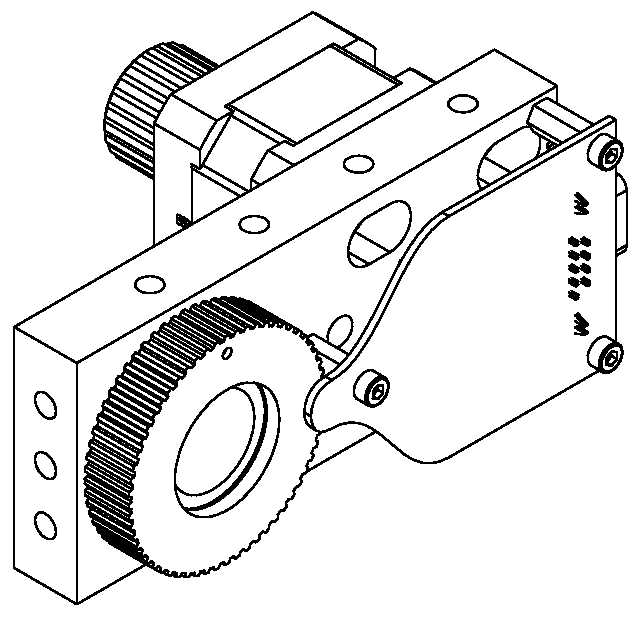
\includegraphics[width=0.65\textwidth]{./drawings/m101_full_dwg.pdf}}


\FloatBarrier
\newpage
\subsection*{Specifications}

\newcolumntype{C}[1]{>{\centering\arraybackslash}p{#1}}
\begin{table}[htbp]
  \centering
  \begin{tabular}{C{2cm} C{2cm} *{3}{C{1cm}} *{3}{C{1cm}} C{1.5cm} }
    \toprule
    \textbf{Parameter} & \textbf{Conditions} &
    \multicolumn{3}{p{3cm}}{\centering\textbf{M101A}} &
    \multicolumn{3}{p{3cm}}{\centering\textbf{M101B}} &
    \textbf{Unit} \\
    \cmidrule(lr){3-5} \cmidrule(lr){6-8}
    & &
    Min & Typ & Max &
    Min & Typ & Max &\\
    \toprule
    Current &  & 0.1 & 1.3 & 1.33 & 0.1 & 1.65 & 1.68 & A/Phase\\ \midrule
    Holding torque & Subst.=1, Curr.=1.33A & & 7 & & & 14.6 & & Ncm \\ \midrule
    Step angle & Subst.=1 & & 0.3 & & & 0.3 & & Degree \\ \midrule
    Step angle accuracy &  & & 1.7 & & & 1.7 & & \% \\ \midrule
    Backlash &  & & 0.1 & & & 0.1 & & deg \\ \midrule
    Gear ratio &  & & 3 & & & 3 & &  \\ \midrule
    Velocity & Subst.=1 & &  & & &  & & deg/s \\ \midrule
    Load capacity &  & &  & & &  & & kg \\ \midrule
    Weight &  & & 0.504 & & & 0.634 & & kg \\ \midrule
    Temperature range &  & -10 &  & 50 & -10 &  & 50 & $^{\circ}$C \\
    \bottomrule
  \end{tabular}
\end{table}

\FloatBarrier
\subsection*{Connection Diagram}
 \begin{minipage}{\textwidth}
  \begin{minipage}[b]{0.49\textwidth}
    \centering
    D-SUB 9 female connector\\
    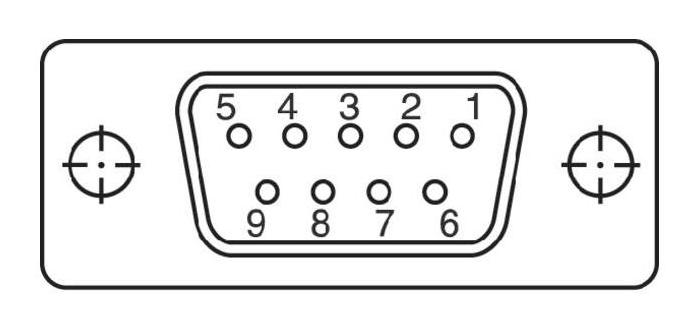
\includegraphics[width=0.65\textwidth]{./drawings/dsub9fem.jpg}\\
    Front view
  \end{minipage}
  \hfill
  \begin{minipage}[b]{0.49\textwidth}
    \begin{tabular}{cc}
      \toprule
      \textbf{Pin} & \textbf{Function} \\
      \toprule
      1 & Phase B1 \\ \midrule
      2 & Phase B2\\ \midrule
      3 & Phase A2 \\ \midrule
      4 & Phase A1 \\ \midrule
      5 & Ground \\ \midrule
      6 & +5V \\ \midrule
      7 & Sens 1 \\ \midrule
      8 & Sens 2 \\ \midrule
      9 & Sens 3 \\ \midrule
      Shield & NC \\
      \bottomrule
    \end{tabular}
  \end{minipage}
\end{minipage}



\FloatBarrier
\begin{figure}
\subsection*{Outline Dimensions}
  \centering
  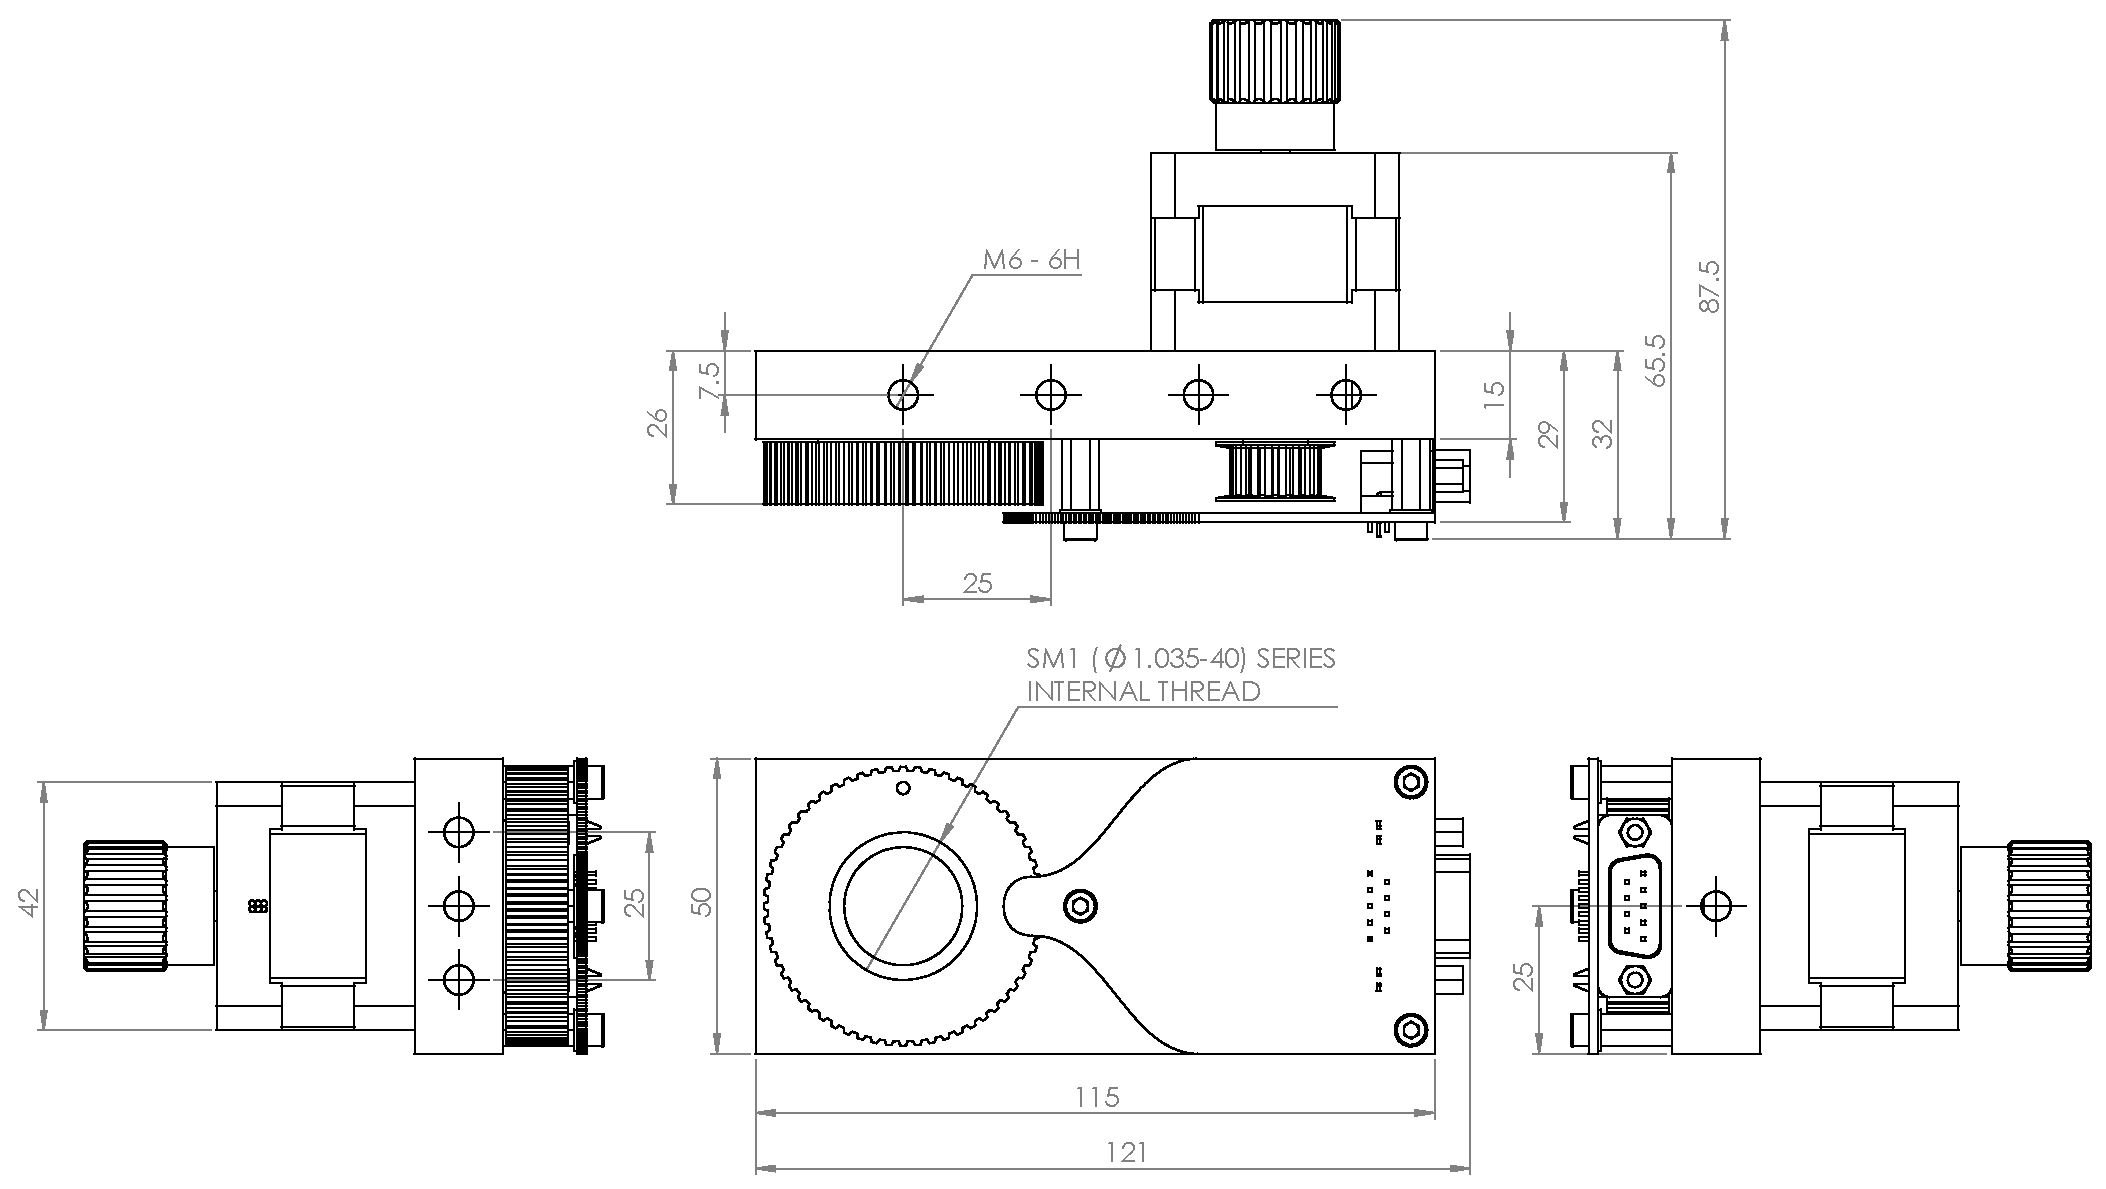
\includegraphics[angle=90,origin=c,width=0.8\textwidth]{./drawings/M101_outline_dimensions.pdf}
\end{figure}
\vfill
\FloatBarrier

\subsection*{Ordering Information}
\begin{tabular}{c|c}
  \hline
  \textbf{Model} & \textbf{Description} \\
  \hline
  M101A   & with knob \\
  M101ANK & without knob \\
  M101B   & with knob \\
  M101BNK & without knob \\
  \hline 
\end{tabular}




\vfill
\end{document}
